
%%%%%%%%%%%%%%%%%%%%%%%%%%%%%%%%%%%%%%%%%%%%%%%%%%%%%%%%%%
%%%%%%%%%%%%%%%%%%%%%%%%%%%%%%%%%%%%%%%%%%%%%%%%%%%%%%%%%%
\chapter{Quantitative Metrics for 2D Packings}
\label{chapter_qualitative_metrics}
%%%%%%%%%%%%%%%%%%%%%%%%%%%%%%%%%%%%%%%%%%%%%%%%%%%%%%%%%%
%%%%%%%%%%%%%%%%%%%%%%%%%%%%%%%%%%%%%%%%%%%%%%%%%%%%%%%%%%


%%%%%%%%%%%%%%%%%%%%%%%%%%%%%%%%%%%%%%%%%%%%%%%%%%%%%%%%%%
%%%%%%%%%%%%%%%%%%%%%%%%%%%%%%%%%%%%%%%%%%%%%%%%%%%%%%%%%%
\section{Introduction}
%%%%%%%%%%%%%%%%%%%%%%%%%%%%%%%%%%%%%%%%%%%%%%%%%%%%%%%%%%
%%%%%%%%%%%%%%%%%%%%%%%%%%%%%%%%%%%%%%%%%%%%%%%%%%%%%%%%%%


\newtext
{
As with many techniques in artistic applications of computer graphics, evaluating the
quality of a computer-generated element packing is a challenge.
The visual appeal of packings follows in part from aligning neighboring elements along compatible 
segments of their boundaries, suggesting that they interlock by design. 
We believe that the evenness of negative space is an indicator 
on how much the elements interlock.
The separation between neighboring elements should be roughly the same everywhere.
%In the limit, as this element separation goes to zero,
%the packing turns into a tessellation: a set of elements that exactly
%fill a container with no overlaps.  
In this chapter, we have developed several measurements of evenness,
which allow us to examine the behavior of manually constructed reference
packings and to compare RepulsionPak with other packing algorithms.
}

%%%%%%%%%%%%%%%%%%%%%%%%%%%%%%%%%%%%%%%%%%%%%%%%%%%%%%%%%%
%%%%%%%%%%%%%%%%%%%%%%%%%%%%%%%%%%%%%%%%%%%%%%%%%%%%%%%%%%
\section{Related Work}
%%%%%%%%%%%%%%%%%%%%%%%%%%%%%%%%%%%%%%%%%%%%%%%%%%%%%%%%%%
%%%%%%%%%%%%%%%%%%%%%%%%%%%%%%%%%%%%%%%%%%%%%%%%%%%%%%%%%%


\newtext
{
%Isenberg has compiled a survey of NPR evaluation~\cite{Isenberg2013},
%but we find that past work in 2D packing evaluation is still limited.
In this section, we discuss a few related methods for evaluating discrete texture synthesis,
stippling, or packings.
For more general discussion, Isenberg compiled a survey of evaluation methods in NPR research~\cite{Isenberg2013}.
%For a compilation of NPR evaluation in general, please refer to a survey by Isenberg~\cite{Isenberg2013}.
}

%To create a good packing, Chapter~\ref{chapter_flowpak} describes
%a few design principles should be followed: balance, flow, uniformity amidst variety, and boundary.
%However, it remains challenging to measure these principles.

%To create a good packing, Chapter~\ref{chapter_flowpak} and Wong et al.~\cite{Wong1998} describe
%a few qualitative principles should be followed: balance, flow, uniformity amidst variety, and boundary.
%%Gieseke et al.~\cite{Gieseke2017} suggested that symmetry is also important.
%However, it remains difficult to measure these principles.
%%Research in NPR is lacking of evaluation, both qualitatively and quantitatively.
%Isenberg has compiled a survey of NPR evaluation~\cite{Isenberg2013}, 
%and we find that past work in 2D packing evaluation is still limited.
%%In this section, we discuss relevant work in qualitative evaluation and quantitative evaluation.
%%A few methods have been proposed for evaluating discrete textures or stippling,
%%but they cannot be extended to our work and past work in 2D packing evaluation is still limited.


\newtext
{
\textbf{Qualitative Evaluation:}
AlMeraj et al.~\cite{AlMerajEval2013} proposed qualitative evaluations to find
the similarity between smaller texture exemplars and bigger synthesized textures.
They conducted two user studies: a pile-sorting study and a pairwise comparison study.
These user studies concerned about small-sized element distributions, but not element interlocking or the evenness of negative space, 
so their work is not suitable for our packing evaluation.
Kwan et al. performed a simple user study of 13 participant to compare 
Pyramid of Arclength Descriptor (PAD)~\cite{Kwan2016} with previous packing methods.
A participant was randomly shown a computer-generated packing and they had to give ratings from 1 (worst) to 6 (best)
to each of three categories: their preference, stylishness, interlocking.
The study revealed that PAD received the highest scores on all three categories.
However, we argue that the first two categories are ambiguous and do not give better understanding to the quality of a packing.
%The study revealed that PAD have the highest scores,
%but the first two factor are questionable and they also omitted element overlaps as a factor.
%We argue that the first two categories are ambiguous and does not give better understanding of the quality of a packing.
%The study revealed that PAD have the highest scores but they overlooked
%other important factors, such as the evenness of negative space or overlaps.
}

\newtext
{
\textbf{Quantitative Evaluation:}
In Jigsaw Image Mosaics (JIM)~\cite{Kim2002}, Kim et al. uses an energy minimization approach
that penalizes a packing if it has too much negative space,
too many overlaps, or severely deformed elements. 
They did not further discuss whether it can be used for a quantitative evaluation,
but we are inspired by their work to develop a metric based on shape overlaps (Section~\ref{section_overlap_function}).
Maciejewski et al.~\cite{Maciejewski2008} compared computer-generated 
with artist-made stipple artwork using the Gray-Level Co-Occurrence Matrix (GLCM),
which measures spatial relationships between pixel intensities.
GLCM works best for analyzing dense point distributions, but it unfortunately cannot be used to analyze arrangements with larger shapes.
In medical research, Aliy et al.~\cite{Aliy2013} proposed a method to analyze small biological objects in a histology image.
They treated these objects as a point distribution by computing their centroids and encoded their spatial relationships, 
so their work is unsuitable for our research.
In fabrication, the packing quality is dictated by manufacturing constraints, such as connectivity,
so that printed objects can resist from breaking~\cite{Chen2016, Zehnder2016, Martinez2019}.
However, our objective is more about the evenness of negative space and less about connectivity strengths.
}


%A few methods have been proposed for evaluating discrete textures or stippling,
%but they cannot be extended to our work and past work in 2D packing evaluation is still limited.

%%%%%%%%%%%%%%%%%%%%%%%%%%%%%%%%%%%%%%%%%%%%%%%%%%%%%%%%%%
%%%%%%%%%%%%%%%%%%%%%%%%%%%%%%%%%%%%%%%%%%%%%%%%%%%%%%%%%%
%\section{Attempts to Measure the Evenness}
%\section{Distance Transforms of Negative Space}
%%%%%%%%%%%%%%%%%%%%%%%%%%%%%%%%%%%%%%%%%%%%%%%%%%%%%%%%%%
%%%%%%%%%%%%%%%%%%%%%%%%%%%%%%%%%%%%%%%%%%%%%%%%%%%%%%%%%%



%\begin{figure}[t]
%\centering
%
\includegraphics[width=1.0\textwidth]{figures/metrics/cs.pdf}
%\caption[A Voronoi diagram of three ``C'' shapes]
%{\label{fig_cs}
%\newtext{
%    A Voronoi diagram of three ``C'' shapes. 
%    The Voronoi boundaries does not capture the shape concavities.
%    If we use discs with the same size to replace the shapes, 
%    the Voronoi diagram will be unchanged.}
%  }
%\end{figure}

% Check 06_evauation_06_27

%\newtext
%{
%In this section, we discuss distance transforms applied on the negative space as they give us a hint of the evenness.
%We also considered an idea of augment distance transforms with two structures: Centroidal area Voronoi diagram and medial axes,
%as they bisect the gaps of negative space.
%In the end we discarded the idea, and this section explains why both structures have underlying issues 
%so that we have to come up with the proposed quantitative metrics.
%}

%\newtext
%{
%\textbf{Distance Transform:} 
%In the context of 2D packing, we define a distance transform as a 2D image whose pixels labelled with distance values. 
%We compute a distance value $d$ as the Euclidean distance to the closest element boundary (Figure~\ref{fig_distance_transform}).
%We only evaluate the distance transform on all pixels inside the negative space.
%Distance $d > 0$ if $\bm{p}$ belongs to the negative space (outside all elements), 
%or $d = 0$ if $p$ belongs to the positive space (inside an element).
%The distance transform gives us a hint about the evenness of negative space.
%An uneven distribution of elements would have significant empty patches,
%causing ``high'' $d$ values locally, which appear as white ridges in Figure~\ref{fig_distance_transform}.
%These ridges are the local maxima of the distance transform. 
%To evaluate the evenness of negative space we can evaluate the values of all local maxima, 
%however, it is not an easy task because the value term of ``local''.
%}


%\newtext
%{
%All $d$ values on the Voronoi cell boundaries can be considered local.
%The spectral packing~\cite{Dalal2006} utilized a centroidal area Voronoi diagram for their optimization approach.
%For each element, they aim to minimize $\sum_{\bm{p} \in I} d^2$,
%where $I$ is the negative space inside the element's Voronoi cell.
%That is, they seek the best alignment of every element with the boundary of its voronoi cell,
%which can be achieved using a Fourier-based correlation.
%However, Voronoi cell boundaries cannot capture local maxima that is created by concave elements,
%hollow concavities of C-shaped elements shown in Figure~\ref{fig_cs} are left out.
%}

%\newtext
%{
%An alternative to handle concave elements is to generate a medial axis from the negative space.
%We define a medial axis as a set of connected point, each should have more than one closest point on element boundaries.
%In Figure~\ref{fig_skeleton}, Medial axis is a superset containing branches that extend to element concavities.
%A medial axis does seem to capture more local maxima than Voronoi cell boundaries.
%However, a medial axis contains problematic branches.
%Many branches extend too far inside sharp concavities so that their ends touch (or almost touch) the element boundaries.
%We also need to prune short unnecessary branches.
%}




%%%%%%%%%%%%%%%%%%%%%%%%%%%%%%%%%%%%%%%%%%%%%%%%%%%%%%%%%%
%%%%%%%%%%%%%%%%%%%%%%%%%%%%%%%%%%%%%%%%%%%%%%%%%%%%%%%%%%
\section{Quantitative Metrics}
%%%%%%%%%%%%%%%%%%%%%%%%%%%%%%%%%%%%%%%%%%%%%%%%%%%%%%%%%%
%%%%%%%%%%%%%%%%%%%%%%%%%%%%%%%%%%%%%%%%%%%%%%%%%%%%%%%%%%

\textbf{Calibration:}
Two packings must be calibrated to each other before our measurements 
can be compared meaningfully.  
We can compare packings of different sizes by normalizing their containers to
have unit area.  We must also arrange for the packings to have the same
\textit{negative space ratio} 
(the overall amount of negative space as a 
fraction of container area), so that our measurements can focus on the
distribution of negative space and not just the amount.  Given two
calibrated packings, we examine three main evenness metrics:
spherical contact probabilities,
distance histograms,
and overlap of offset elements. 


%%%%%%%%%%%%%%%%%%%%%%%%%%%%%%%%%%%%%%%%%%%%%%%%%%%%%%%%%%
%%%%%%%%%%%%%%%%%%%%%%%%%%%%%%%%%%%%%%%%%%%%%%%%%%%%%%%%%%
\subsection{Spherical Contact Probability}
%%%%%%%%%%%%%%%%%%%%%%%%%%%%%%%%%%%%%%%%%%%%%%%%%%%%%%%%%%
%%%%%%%%%%%%%%%%%%%%%%%%%%%%%%%%%%%%%%%%%%%%%%%%%%%%%%%%%%

The spherical contact probability (SCP) is the probability that a 
disc of radius $r$, chosen
uniformly at random within the container region, lies entirely within the 
packing's negative space~\cite{Chiu2013}.
The SCP can be summarized via a function $Q_s(r)$ that gives this 
probability for each radius $r$.
In order to interpret the SCP, it is helpful first to
examine a ``packing'' with perfectly even negative space (Figure~\ref{hsr_viz}a).
Consider a pattern of infinite horizontal stripes of width $d_\mathrm{s}$,
\newtext{separated from each other by negative space of width $d_\mathrm{gap}$}.  For this pattern,
$Q_s(0)=d_\mathrm{gap}/(d_\mathrm{gap}+d_\mathrm{s})$; it is also
clear that $Q_s(d_\mathrm{gap}/2)=0$, because no disc of diameter greater
than $d_\mathrm{gap}$ can fit in the negative space
(our $d_\mathrm{gap}$ is twice the radius of the ball).
Furthermore,
$Q_s(r)$ will decrease linearly between these two points, and remain
at zero thereafter; its graph will consist of a tilted line segment
connected to a horizontal ray.




No real-world packing exhibits this SCP.  Even in a perfect arrangement
of squares (Figure~\ref{hsr_viz}b), the intersections of horizontal and
vertical channels
produce pockets of negative space that can accommodate balls of
radius $d_\mathrm{gap}\sqrt{2}/2$.  These pockets tend to raise the SCP
slightly everywhere, and cause it to bend into a small tail that
approaches zero gradually.
For a given set of elements in a container, the best packings will
have a steeply-decreasing SCP that stays close to the idealized stripe function most
of the way down, has a low value at $r=d_\mathrm{gap}/2$,
and then bends towards horizontal near that value.
Note that there is always a largest disc that can fit in a packing's
negative space, and hence a largest $r$ for which $Q_s(r)>0$.  
In our graphs, we plot $Q_s(r)$ only until this point, allowing us
to compare the largest empty gaps of two packings.
In less effective packings (Figs.~\ref{hsr_viz}c,d), the negative space 
will be narrower in
some places and wider in others, recognizable as a shallower SCP
with a longer tail.

We geometrically compute SCP by offsetting the negative
space inward.  Let $N$ be the shape of the negative space (essentially
the container region with holes where elements are).  For a given radius
$r$, we compute $N(r)$, the Minkowski difference of $N$ with a disc of
radius $r$.  Then $Q_s(r)$ is simply the ratio of the area of $N(r)$ to
the area of the container.

\begin{figure}[h]
\centering
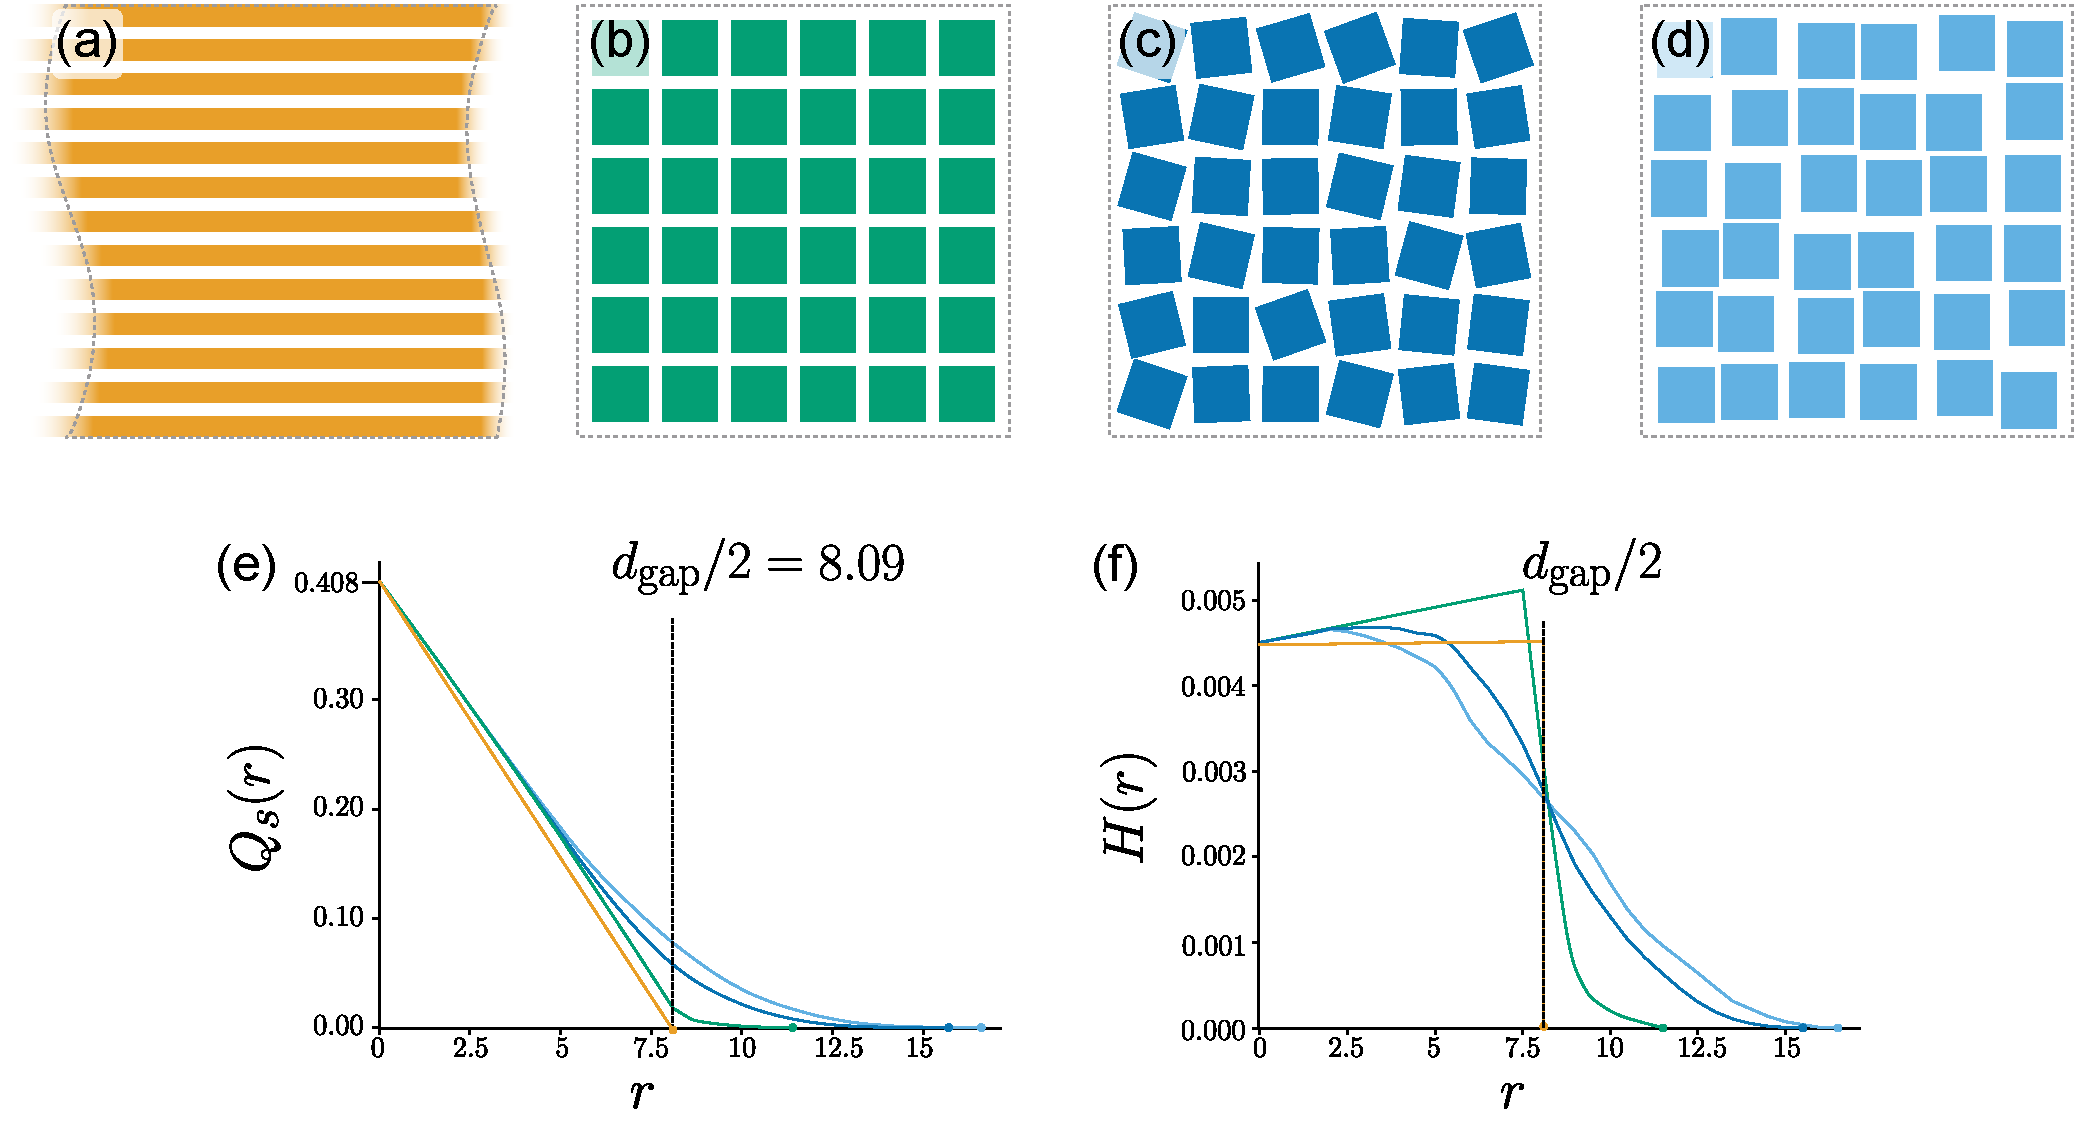
\includegraphics[width=1.0\textwidth]{figures/metrics/hsr_viz_big.pdf}
\caption[Spherical contact probabilities and distance histograms \newline for reference packings]
{\label{hsr_viz}
Spherical contact probabilities and distance histograms for 
reference packings.
A ``perfect packing'' of infinite stripes is shown in~(a),
followed by a square packing with the same area fraction and \newtext{negative space width $d_\mathrm{gap}$}
in~(b).  The square packing is then perturbed with random rotations in~(c)
and translations in~(d). The corresponding SCP functions and histograms are plotted
in~(e) and~(f).}
\end{figure}


%%%%%%%%%%%%%%%%%%%%%%%%%%%%%%%%%%%%%%%%%%%%%%%%%%%%%%%%%%
%%%%%%%%%%%%%%%%%%%%%%%%%%%%%%%%%%%%%%%%%%%%%%%%%%%%%%%%%%
\subsection{Histograms of the Distance Transform}
%%%%%%%%%%%%%%%%%%%%%%%%%%%%%%%%%%%%%%%%%%%%%%%%%%%%%%%%%%
%%%%%%%%%%%%%%%%%%%%%%%%%%%%%%%%%%%%%%%%%%%%%%%%%%%%%%%%%%

\begin{figure}
\centering
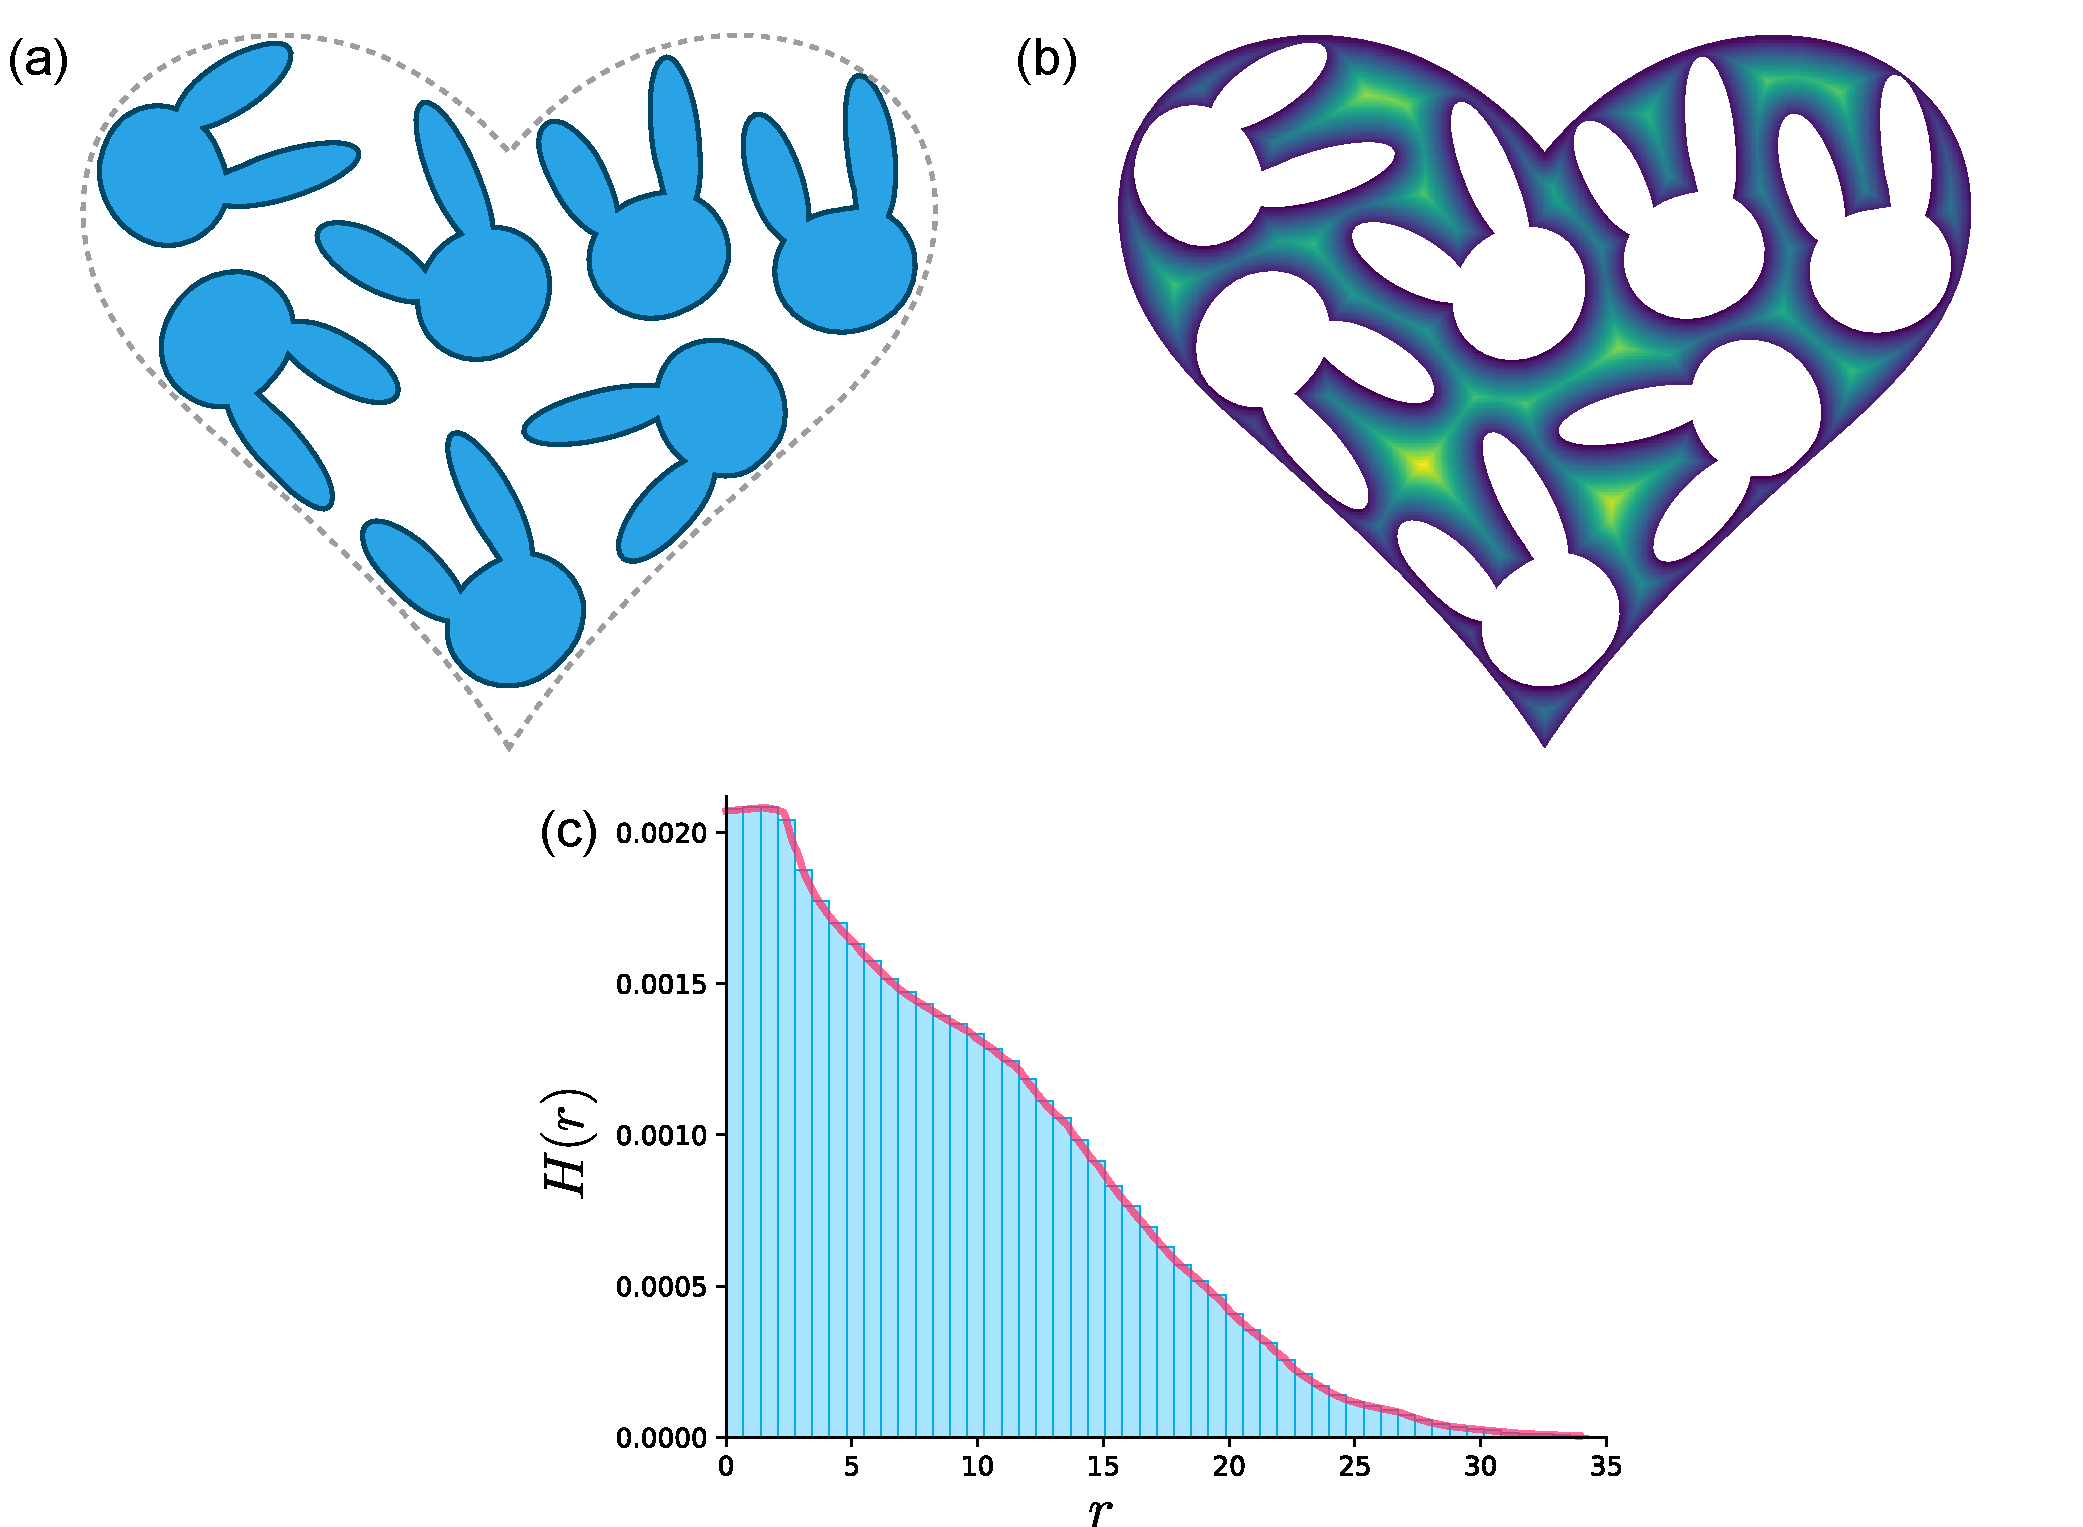
\includegraphics[width=1.0\textwidth]{figures/metrics/rabbit.pdf}
\caption[An example of distance transform of negative space]
{\label{fig_distance_transform}
\newtext{
    The image on the right is a distance transform generated from negative space around two rabbits.
    The brighter the color of a pixel, the farther it is from the nearest boundary.}
  }
\bigskip
\bigskip
\bigskip

\includegraphics[width=1.0\textwidth]{figures/metrics/unilever_with_skeleton_small.pdf}
\caption[An example of a medial axis of negative space]
{\label{fig_skeleton}
\newtext{
    A medial axis generated from the negative space of the Unilever packing using
    \mbox{Zhang-Suen} thinning algorithm~\cite{Zhang1984}.
    The medial axis contains unnecessarily long branches that touch the element boundaries and 
    inconsequential short branches that should be deleted.
  }
}
\end{figure}


\newtext{
The distance transform of the negative space provides insights into how negative space varies. 
In the context of 2D packings, a distance transform is a 2D image where each pixel
contains the radius $r$ value from the nearest element.
Figure~\ref{fig_distance_transform} shows an example for a distance transform,
lighter a color of a pixel, higher the $r$ value. %, showing a pattern of white ridges
%that correspond to a medial axis.
We investigated the idea of analyzing $r$ values only on a medial axis 
since it bisects the gaps of negative space.
%since they can be considered as the widths of negative space gaps.
However, creating a high quality medial axis is difficult,
as shown in Figure~\ref{fig_skeleton}, the challenge is to prune a large number of problematic branches
that are either too long or too short.
}


\newtext
{A histogram of all $r$ values is a better way to analyze the distance transform.}
%{We decide to analyze the entire negative space by generating a histogram of all $r$ values.}
%The distance transform of the negative space can 
%provide insights into how negative space varies
We could calculate a standard \textbf{histogram of the
distance transform}, but that would require quantizing \newtext{$r$ values} into bins.
Instead, note that the SCP $Q_s(r)$ is precisely the normalized area of 
negative space for which the distance transform is at least $r$. 
Looked at another way, if we offset each element by a
radius $r$, then $1-Q_s(r)$ must be the normalized 
area of the union of these offset elements.
% Looked at
% another way, we can offset each element by a radius $r$, in which case 
% $1-Q_s(r)$ must be the normalized area of the union of these offset elements.
This area can then be interpreted as 
a cumulative distribution function of distance.  From this observation
we can compute a continuous variant of the distance histogram as a 
probability density function via the derivative of the SCP: $H(r)=-Q_s'(r)$.


Given two calibrated packings, the areas under their distance histograms
are the same.  But a more even packing will have a shorter tail,
indicating a tighter upper bound on gap size, and it will have a larger
concentration of density around $d_\mathrm{gap}/2$.  In Figure~\ref{hsr_viz},
the histogram for the perfect stripe pattern is a step function that drops
to zero at $d_\mathrm{gap}/2$.  The ideal square packing has a histogram
that climbs gently until around $d_\mathrm{gap}/2$ before dropping
steeply.  The other two packings have shallower, smoother histograms.
Note also that high values of the distance histogram near $d_\mathrm{gap}/2$
correspond to a rapid negative change in the SCP, suggesting a more even
packing.




%%%%%%%%%%%%%%%%%%%%%%%%%%%%%%%%%%%%%%%%%%%%%%%%%%%%%%%%%%
%%%%%%%%%%%%%%%%%%%%%%%%%%%%%%%%%%%%%%%%%%%%%%%%%%%%%%%%%%
\subsection{The Overlap Function}
\label{section_overlap_function}
%%%%%%%%%%%%%%%%%%%%%%%%%%%%%%%%%%%%%%%%%%%%%%%%%%%%%%%%%%
%%%%%%%%%%%%%%%%%%%%%%%%%%%%%%%%%%%%%%%%%%%%%%%%%%%%%%%%%%

\begin{figure}
\centering
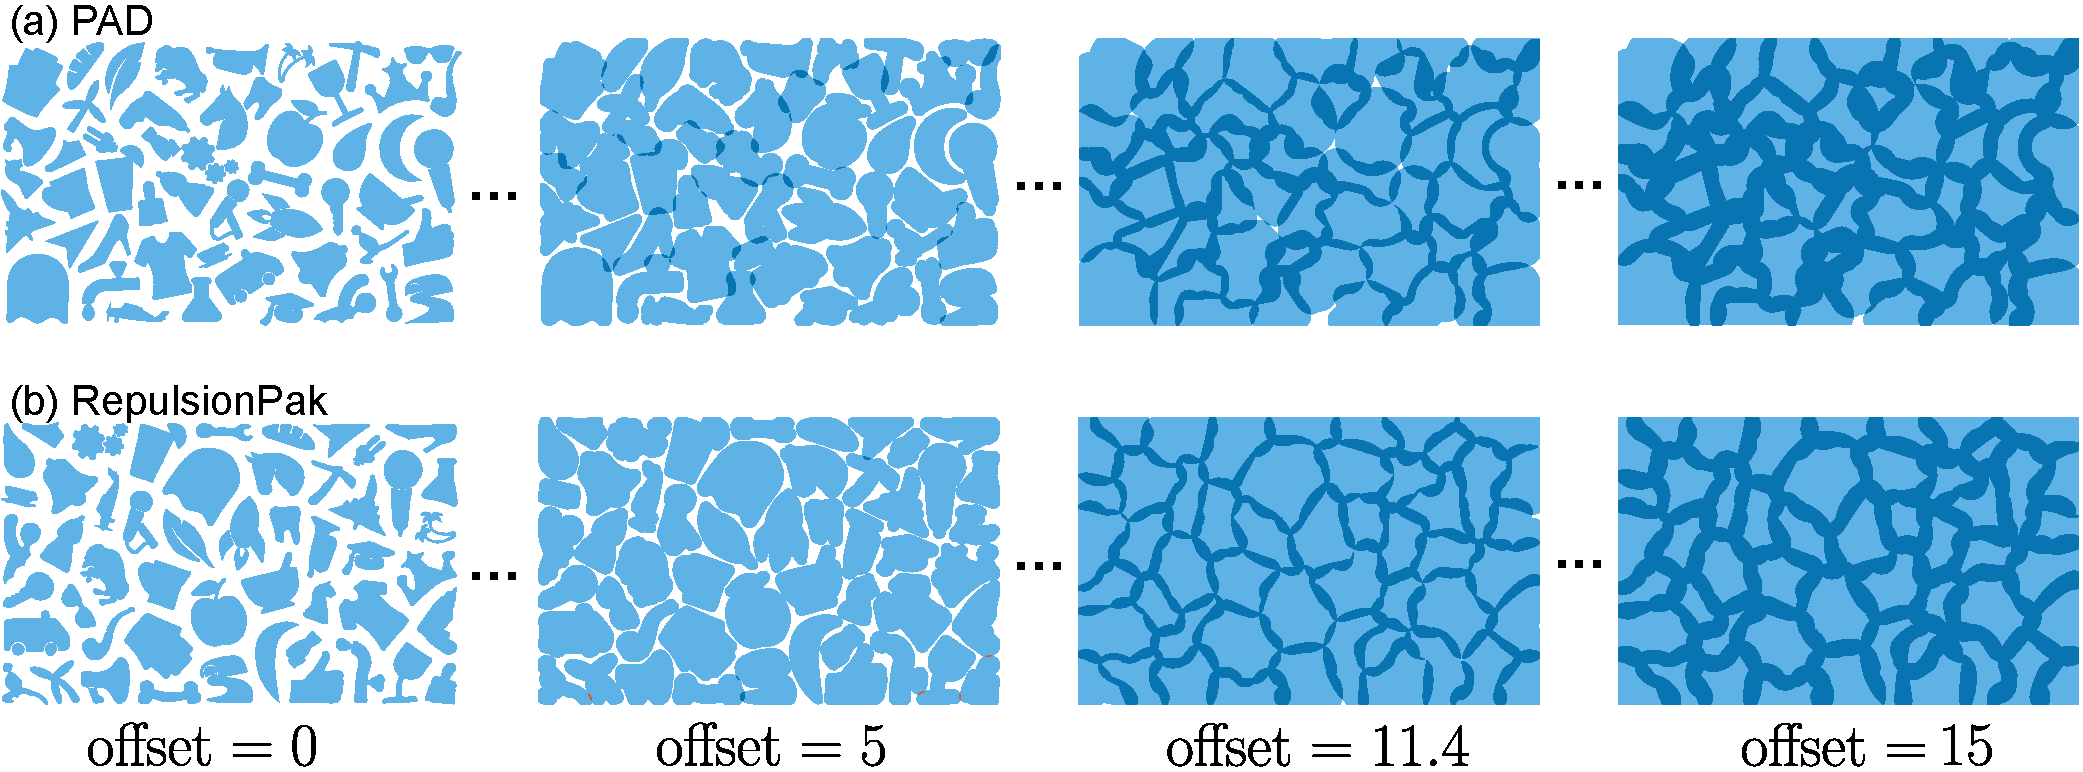
\includegraphics[width=1.0\textwidth]{figures/metrics/overlap_metric.pdf}
\caption[An illustration of offsetting elements outward]
{\label{fig_overlap_function}
    An illustration of offsetting elements outward. The packings have $d_\mathrm{gap} / 2 = 5.7$.  
    At an offset of 5, which is slightly less than $d_\mathrm{gap} / 2$,
    the overlap for the PAD packing is 1.462\% of the total area, while the overlap for our packing is only 0.039\%.
    At an offset of 11.4, which equals $d_\mathrm{gap}$, the PAD packing shows more empty space (1.05\%) than RepulsionPak (0.07\%).
    As the offset is increased, overlaps in the PAD packing create channels
  with uneven widths, whereas ours are more uniform.
  }
\end{figure}

The overlap function is a function of a non-negative offset amount
$r$.  For any given $r$, we offset every element by computing its Minkowski
sum with a disc of radius $r$.  As $r$ grows, elements will start overlapping;
the overlap function measures the total area of these overlaps, normalized
by container area, as a function of $r$.  We can also visualize these 
overlapping areas directly as in Figure~\ref{fig_overlap_function}.  In a 
perfect packing, we would expect no overlaps until $r=d_\mathrm{gap}/2$,
our desired gap distance, at which point overlapping areas would start to
grow into channels of roughly even width.



%%%%%%%%%%%%%%%%%%%%%%%%%%%%%%%%%%%%%%%%%%%%%%%%%%%%%%%%%%
%%%%%%%%%%%%%%%%%%%%%%%%%%%%%%%%%%%%%%%%%%%%%%%%%%%%%%%%%%
\section{Comparisons}
%%%%%%%%%%%%%%%%%%%%%%%%%%%%%%%%%%%%%%%%%%%%%%%%%%%%%%%%%%
%%%%%%%%%%%%%%%%%%%%%%%%%%%%%%%%%%%%%%%%%%%%%%%%%%%%%%%%%%

\newtext
{
	For all comparisons below, 
	we estimate $d_\mathrm{gap}/2$ as the average of skin widths of all elements 
	in a RepulsionPak packing after the simulation stops.
	We assume the other non-RepulsionPak packing has approximately the same $d_\mathrm{gap}/2$ value 
	since both packings have the identical negative space ratio due to the calibration.
}

\textbf{Comparison to PAD:} 
Figure~\ref{pad_comparison} compares
RepulsionPak and PAD~\cite{Kwan2016}.  Packing (a) is
a result from the PAD\ paper; Packing (b) was created with RepulsionPak using
the same elements, and calibrated to have the same negative space as~(a).
Note that the PAD\ packing actually has several overlapping elements
(for example, the tooth and the horse), but white haloes around
elements artfully conceal overlaps with little degradation in
visual quality.  Our packing avoids overlaps by design.
The SCP plot in~(c) shows that our packing has a lower value at $d_\mathrm{gap}/2$,
indicating more even negative space, and has a shorter tail,
indicating fewer large empty areas.
Our result also has a histogram bump around $d_\mathrm{gap}/2$, and 
a lower overlap function.

\begin{figure}
\centering
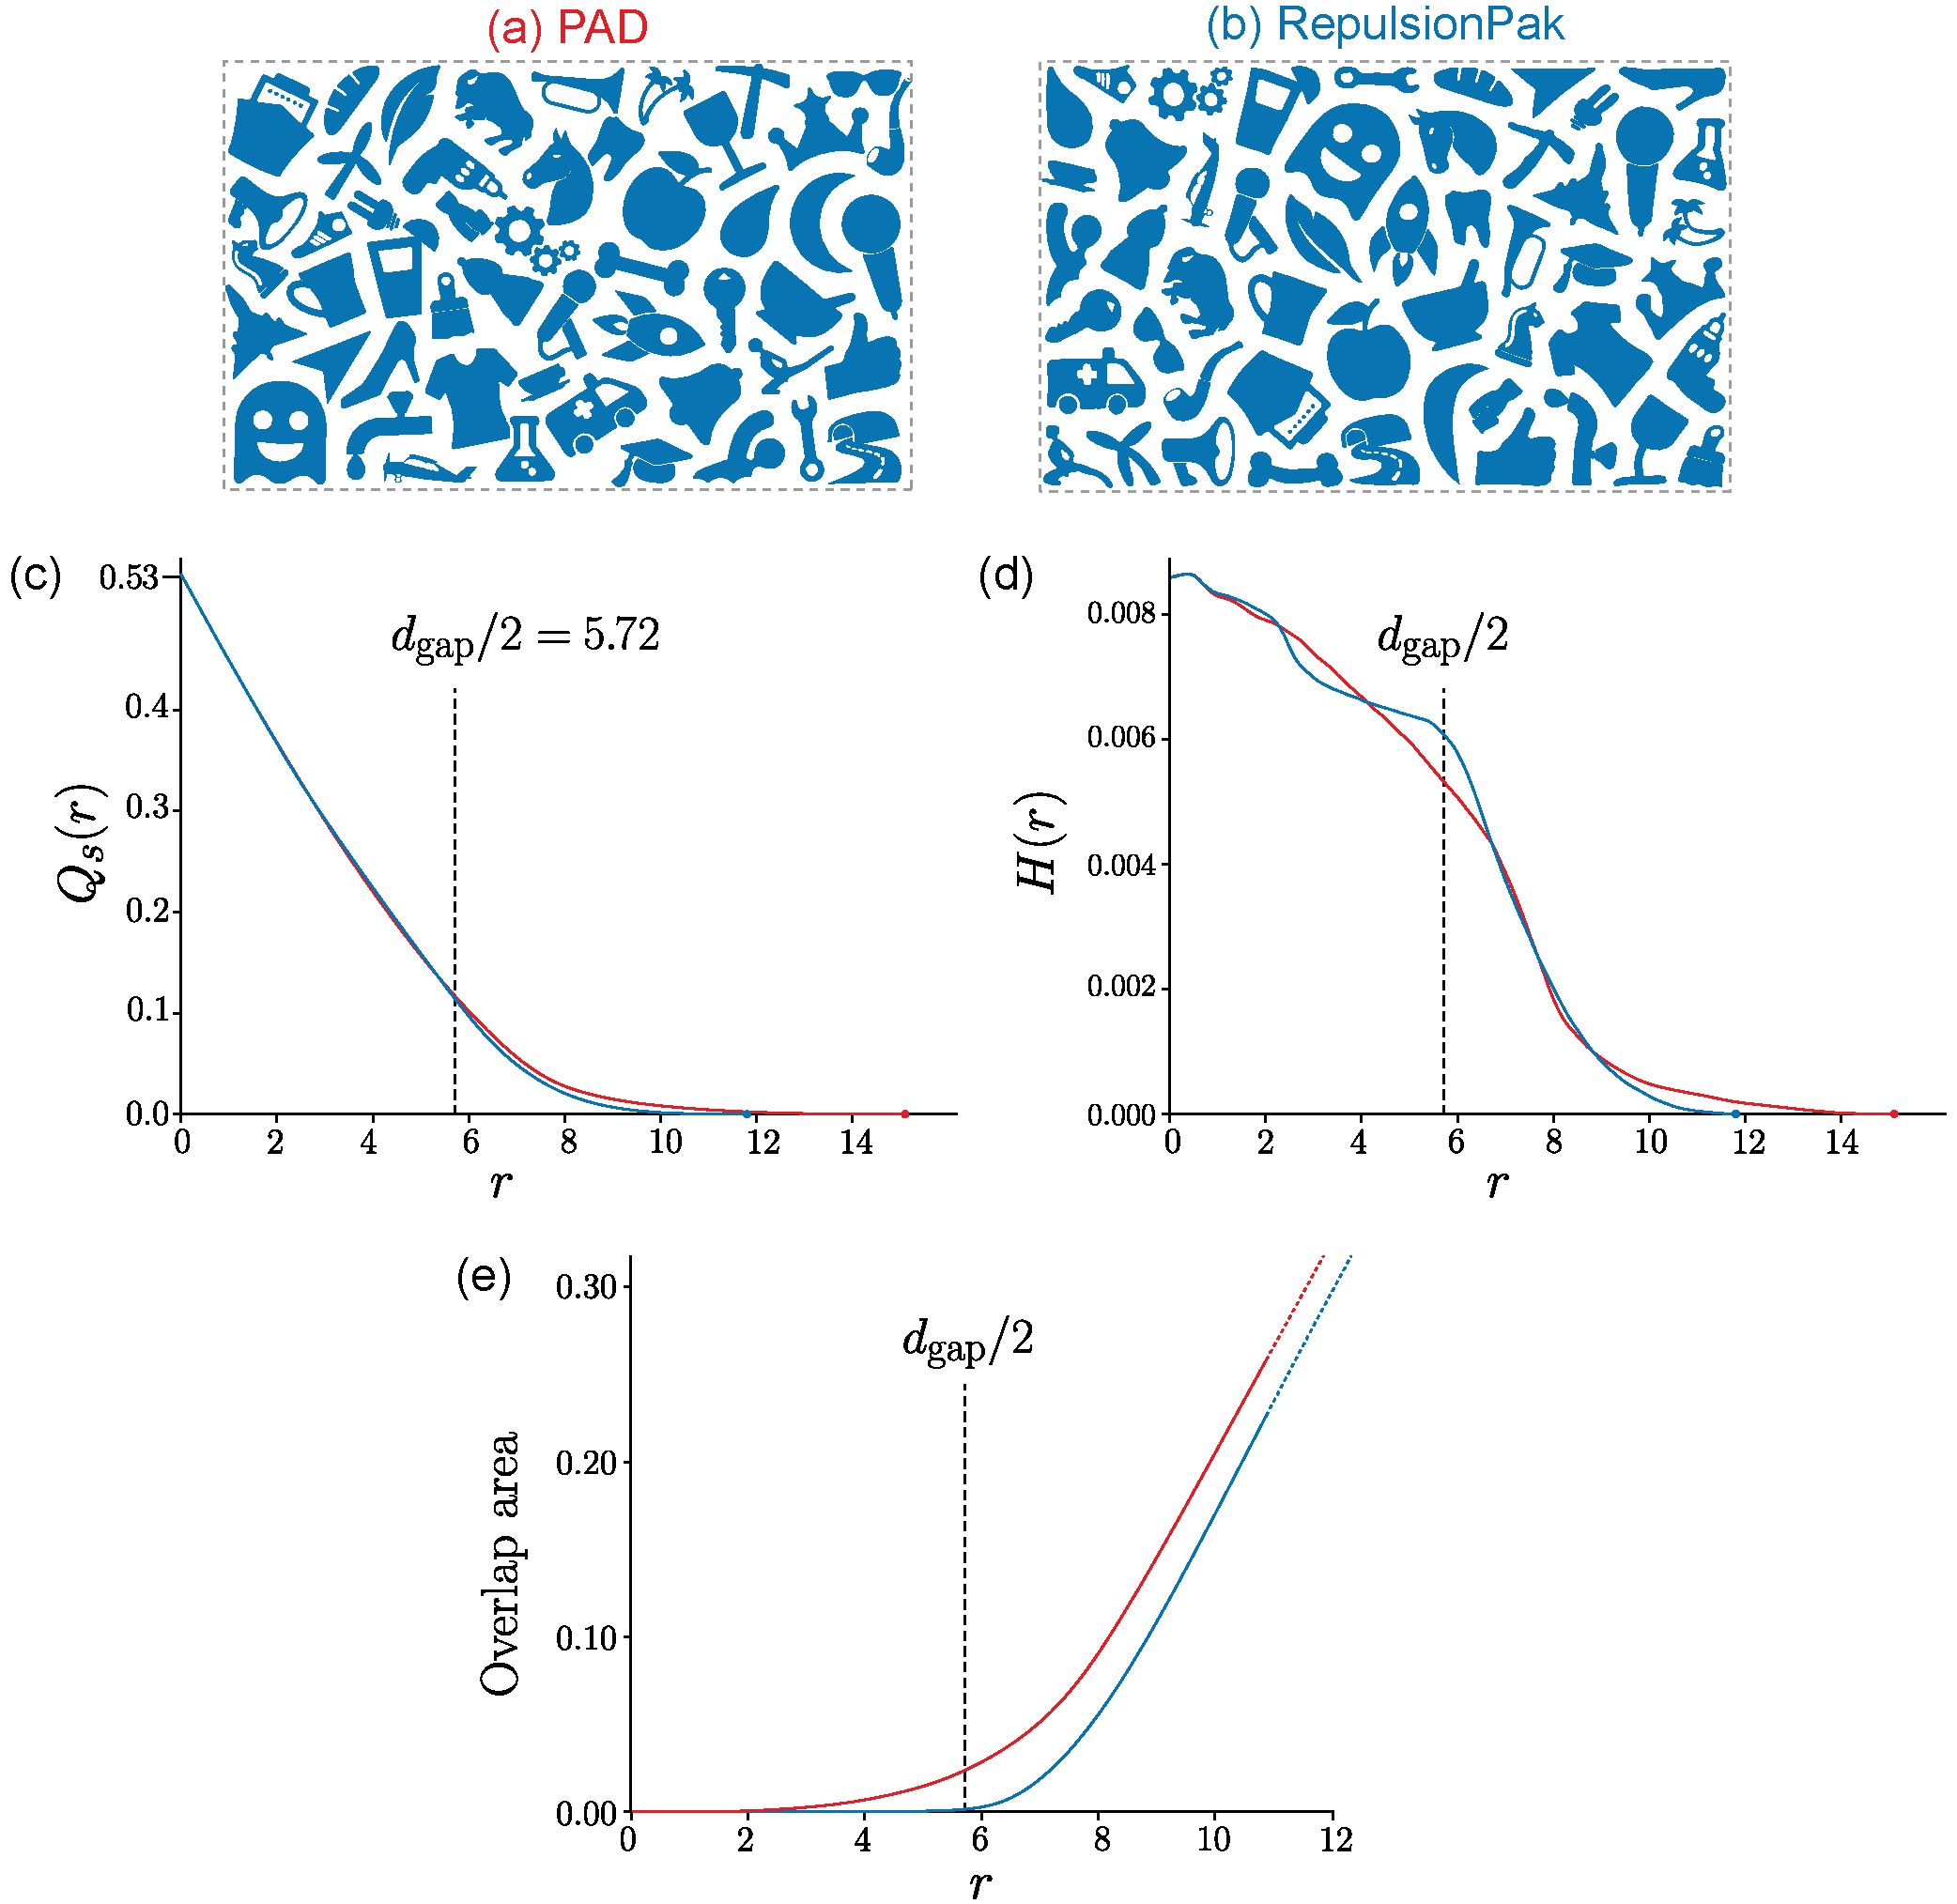
\includegraphics[width=1.0\textwidth]{figures/metrics/pad_comparison_big.pdf}
\caption[A comparison between a PAD~packing and a RepulsionPak packing]
{\label{pad_comparison}
A comparison between a PAD~packing shown in~(a) and a RepulsionPak packing in~(b) 
with their corresponding SCPs~(c), distance histograms~(d), and overlap functions~(e). 
The PAD and RepulsionPak packings are calibrated
to have the same negative space ratio.
Our SCP is lower and shorter than the PAD's result,
our histogram shows higher concentration around $d_\mathrm{gap} / 2$,
indicating more even negative space,
and our packing has a lower overlap function.
}
\end{figure}


\textbf{Comparison to an Artist-Made Packing:} 
In Figure~\ref{balabolka_comparison} we show a RepulsionPak result created 
using the elements from the artist-made packing.
Our packing was calibrated to match the artist's.
Looking closely, the artist's packing has a few elements 
separated by narrow gaps, such as the cherries and the corn on the top left.
Our result has fewer large empty gaps, as indicated by a short tail
in its SCP.
Our result also has a histogram bump around $d_\mathrm{gap}/2$, and a lower overlap function.
The result shows the effectiveness of the repulsion forces in successfully
discovering compatibilities in the element boundaries and filling the space effectively.

\begin{figure}
\centering
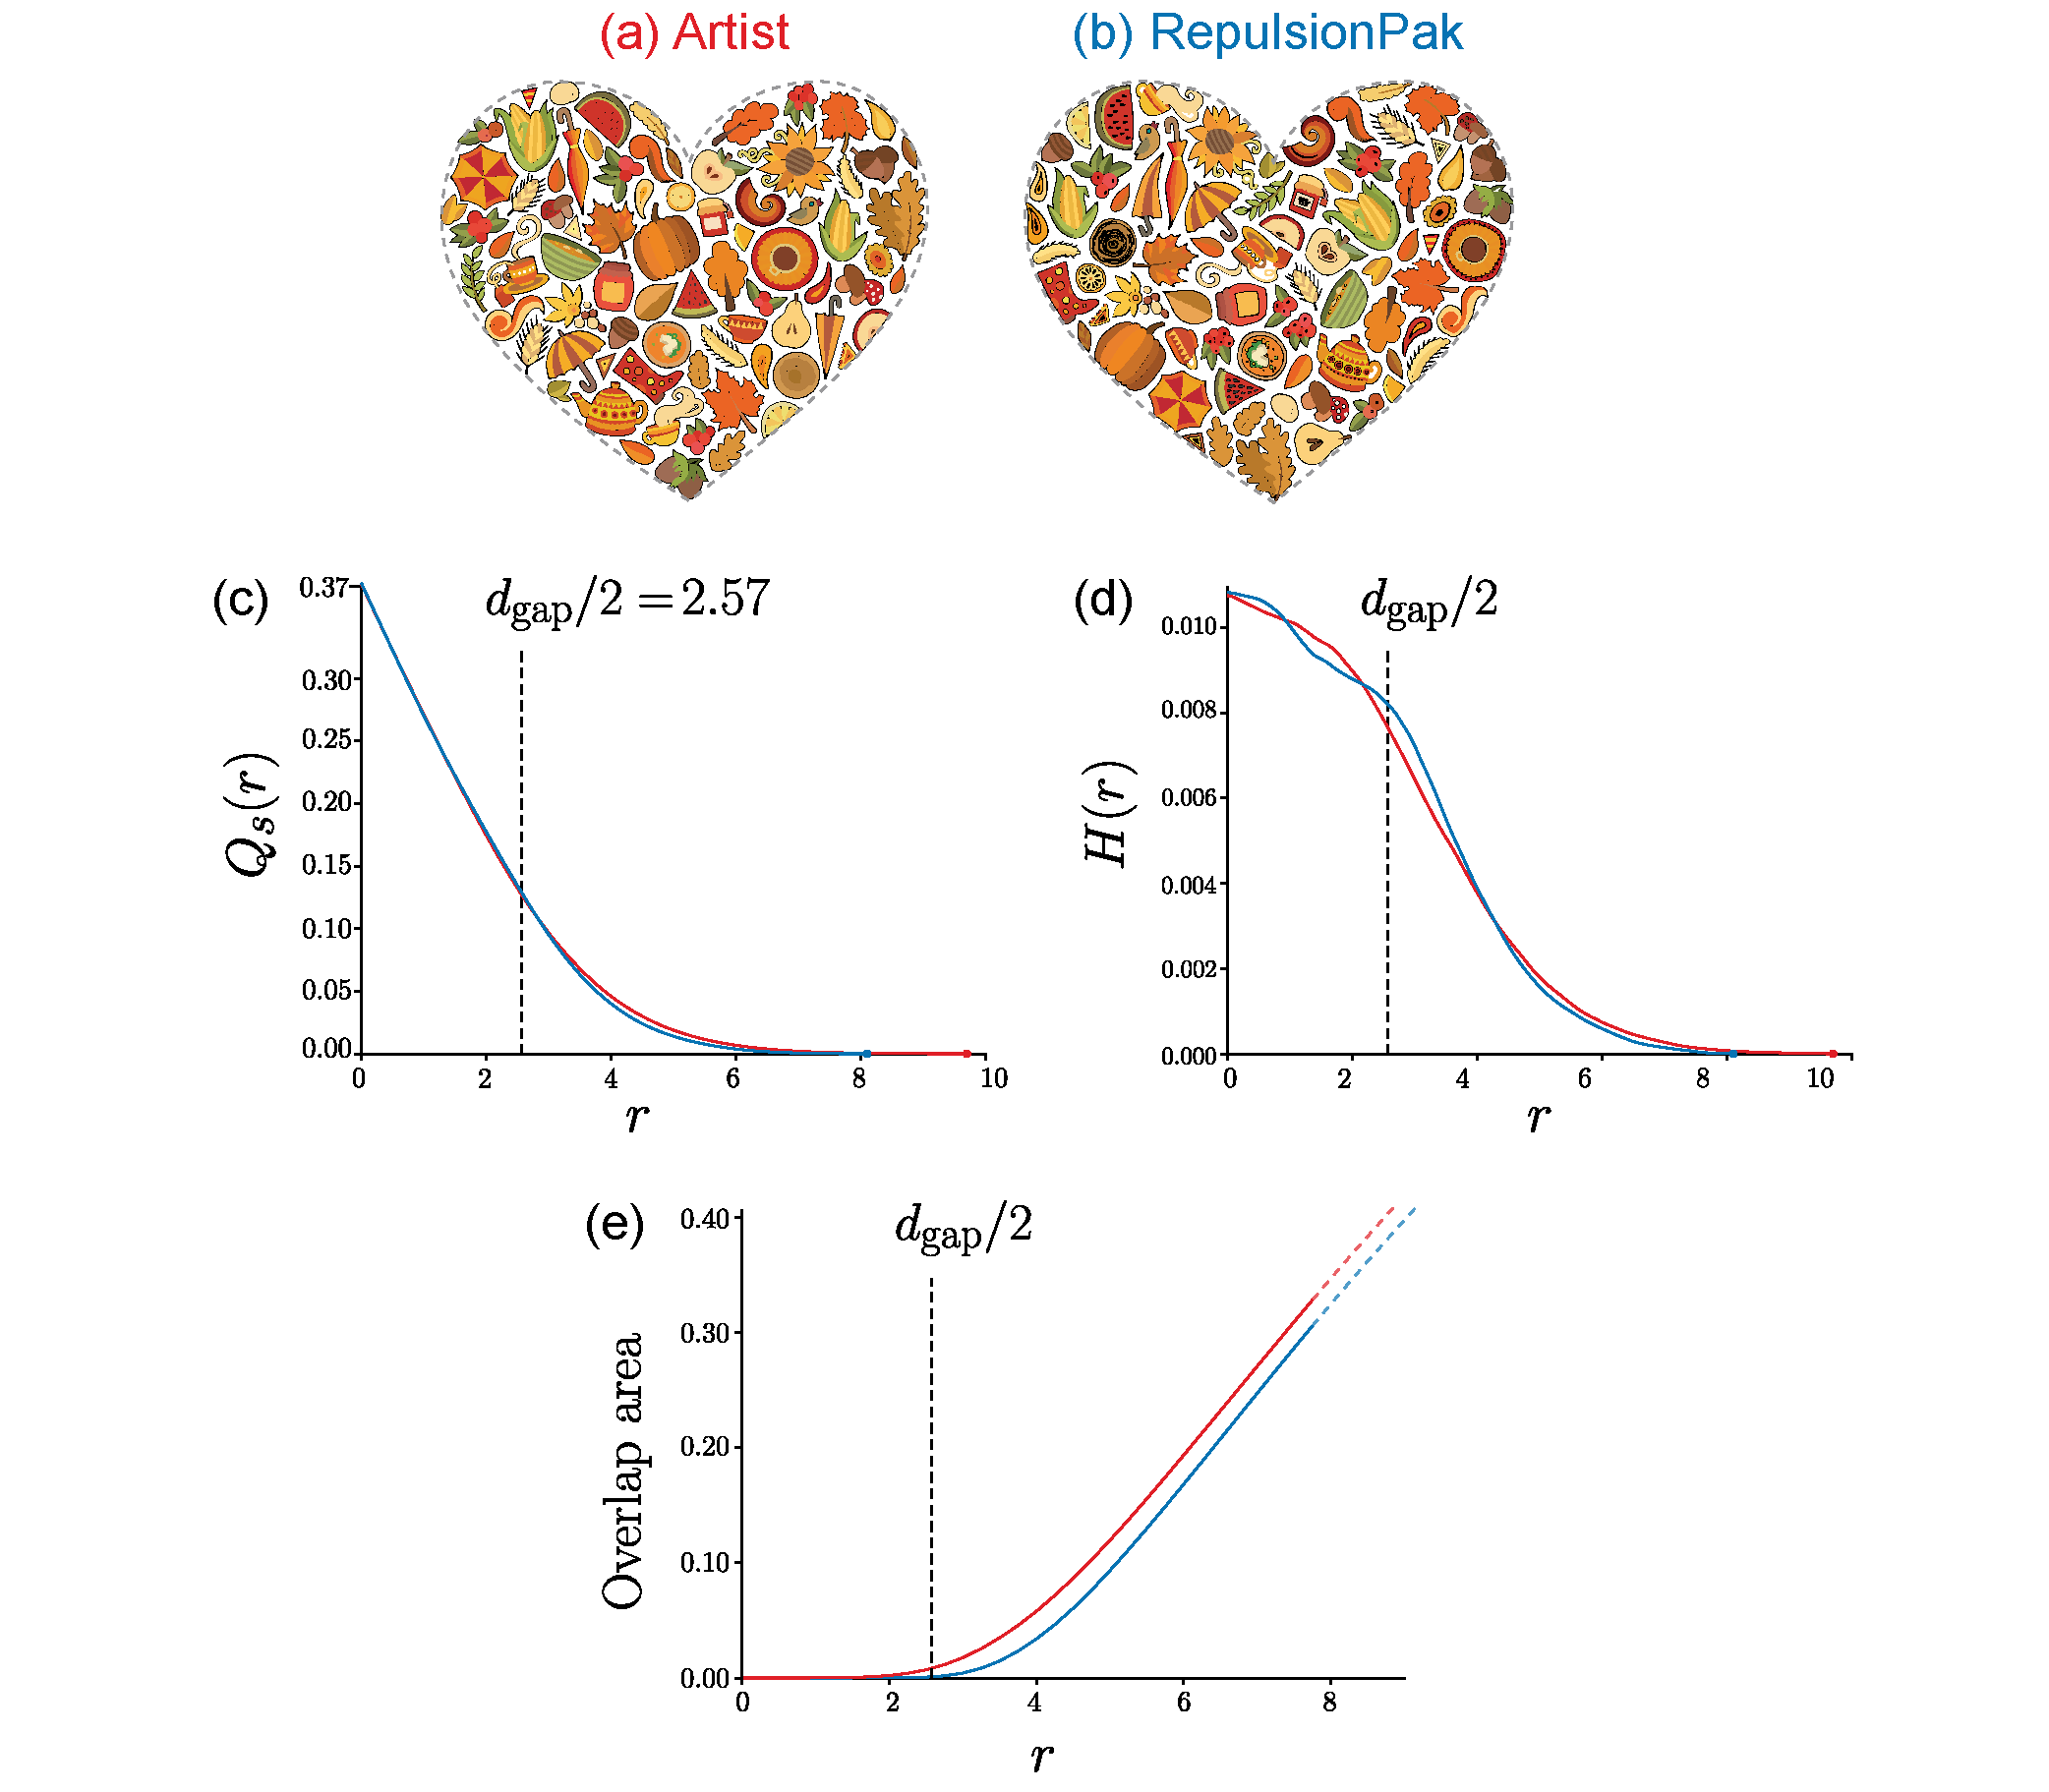
\includegraphics[width=1.0\textwidth]{figures/metrics/balabolka_comparison_big.pdf}
\caption[A comparison between the artist-made packing \newline  and a RepulsionPak packing]
{ \label{balabolka_comparison} 
A comparison between the artist-made packing (Artist: Balabolka on Shutterstock) shown in~(a), and a RepulsionPak packing
with the same elements in~(b).  We plot the corresponding SCPs~(c),
distance histograms~(d), and overlap functions~(e).
For comparison purposes we remove secondary elements from the artist's
packing.  Our SCP is lower and shorter than the artist's result,
our histogram shows more concentration around $d_\mathrm{gap} / 2$,
and RepulsionPak also has a lower overlap function.
}
\end{figure}

\textbf{Comparison to Rigid Packings}: 
To evaluate the effect of deformation on negative space, we compute all three metrics under
increasing values of \newtext{$k_\mathrm{edg}$, the edge force relative strength}.  
\newtext{Note that we only modify the strengths of edge springs and shear springs, 
and the strength of negative space springs are unchanged.}
Increasing $k_\mathrm{edg}$
allows the element meshes to resist deformation, ultimately
approximating a rigid packing algorithm.  We created 15 packings,
five for each of three values of $k_\mathrm{edg}$ (5, 250, and 1000).  Each packing
used 25 elements chosen at random from a library of 60, with
no secondary elements.  
All packings are partly calibrated: they all have the same negative
space ratio, but elements are chosen at random and have some
variation in their sizes.
As shown in Figure~\ref{fifteen_packings}, a low value of
$k_\mathrm{edg}$ leads to greater deformation and steeper SCPs.
The more pronounced histogram bump at $r=d_\mathrm{gap}/2$ suggests
more even negative space.
The lower overlap functions indicate fewer narrow gaps between elements.

\begin{figure}
\centering
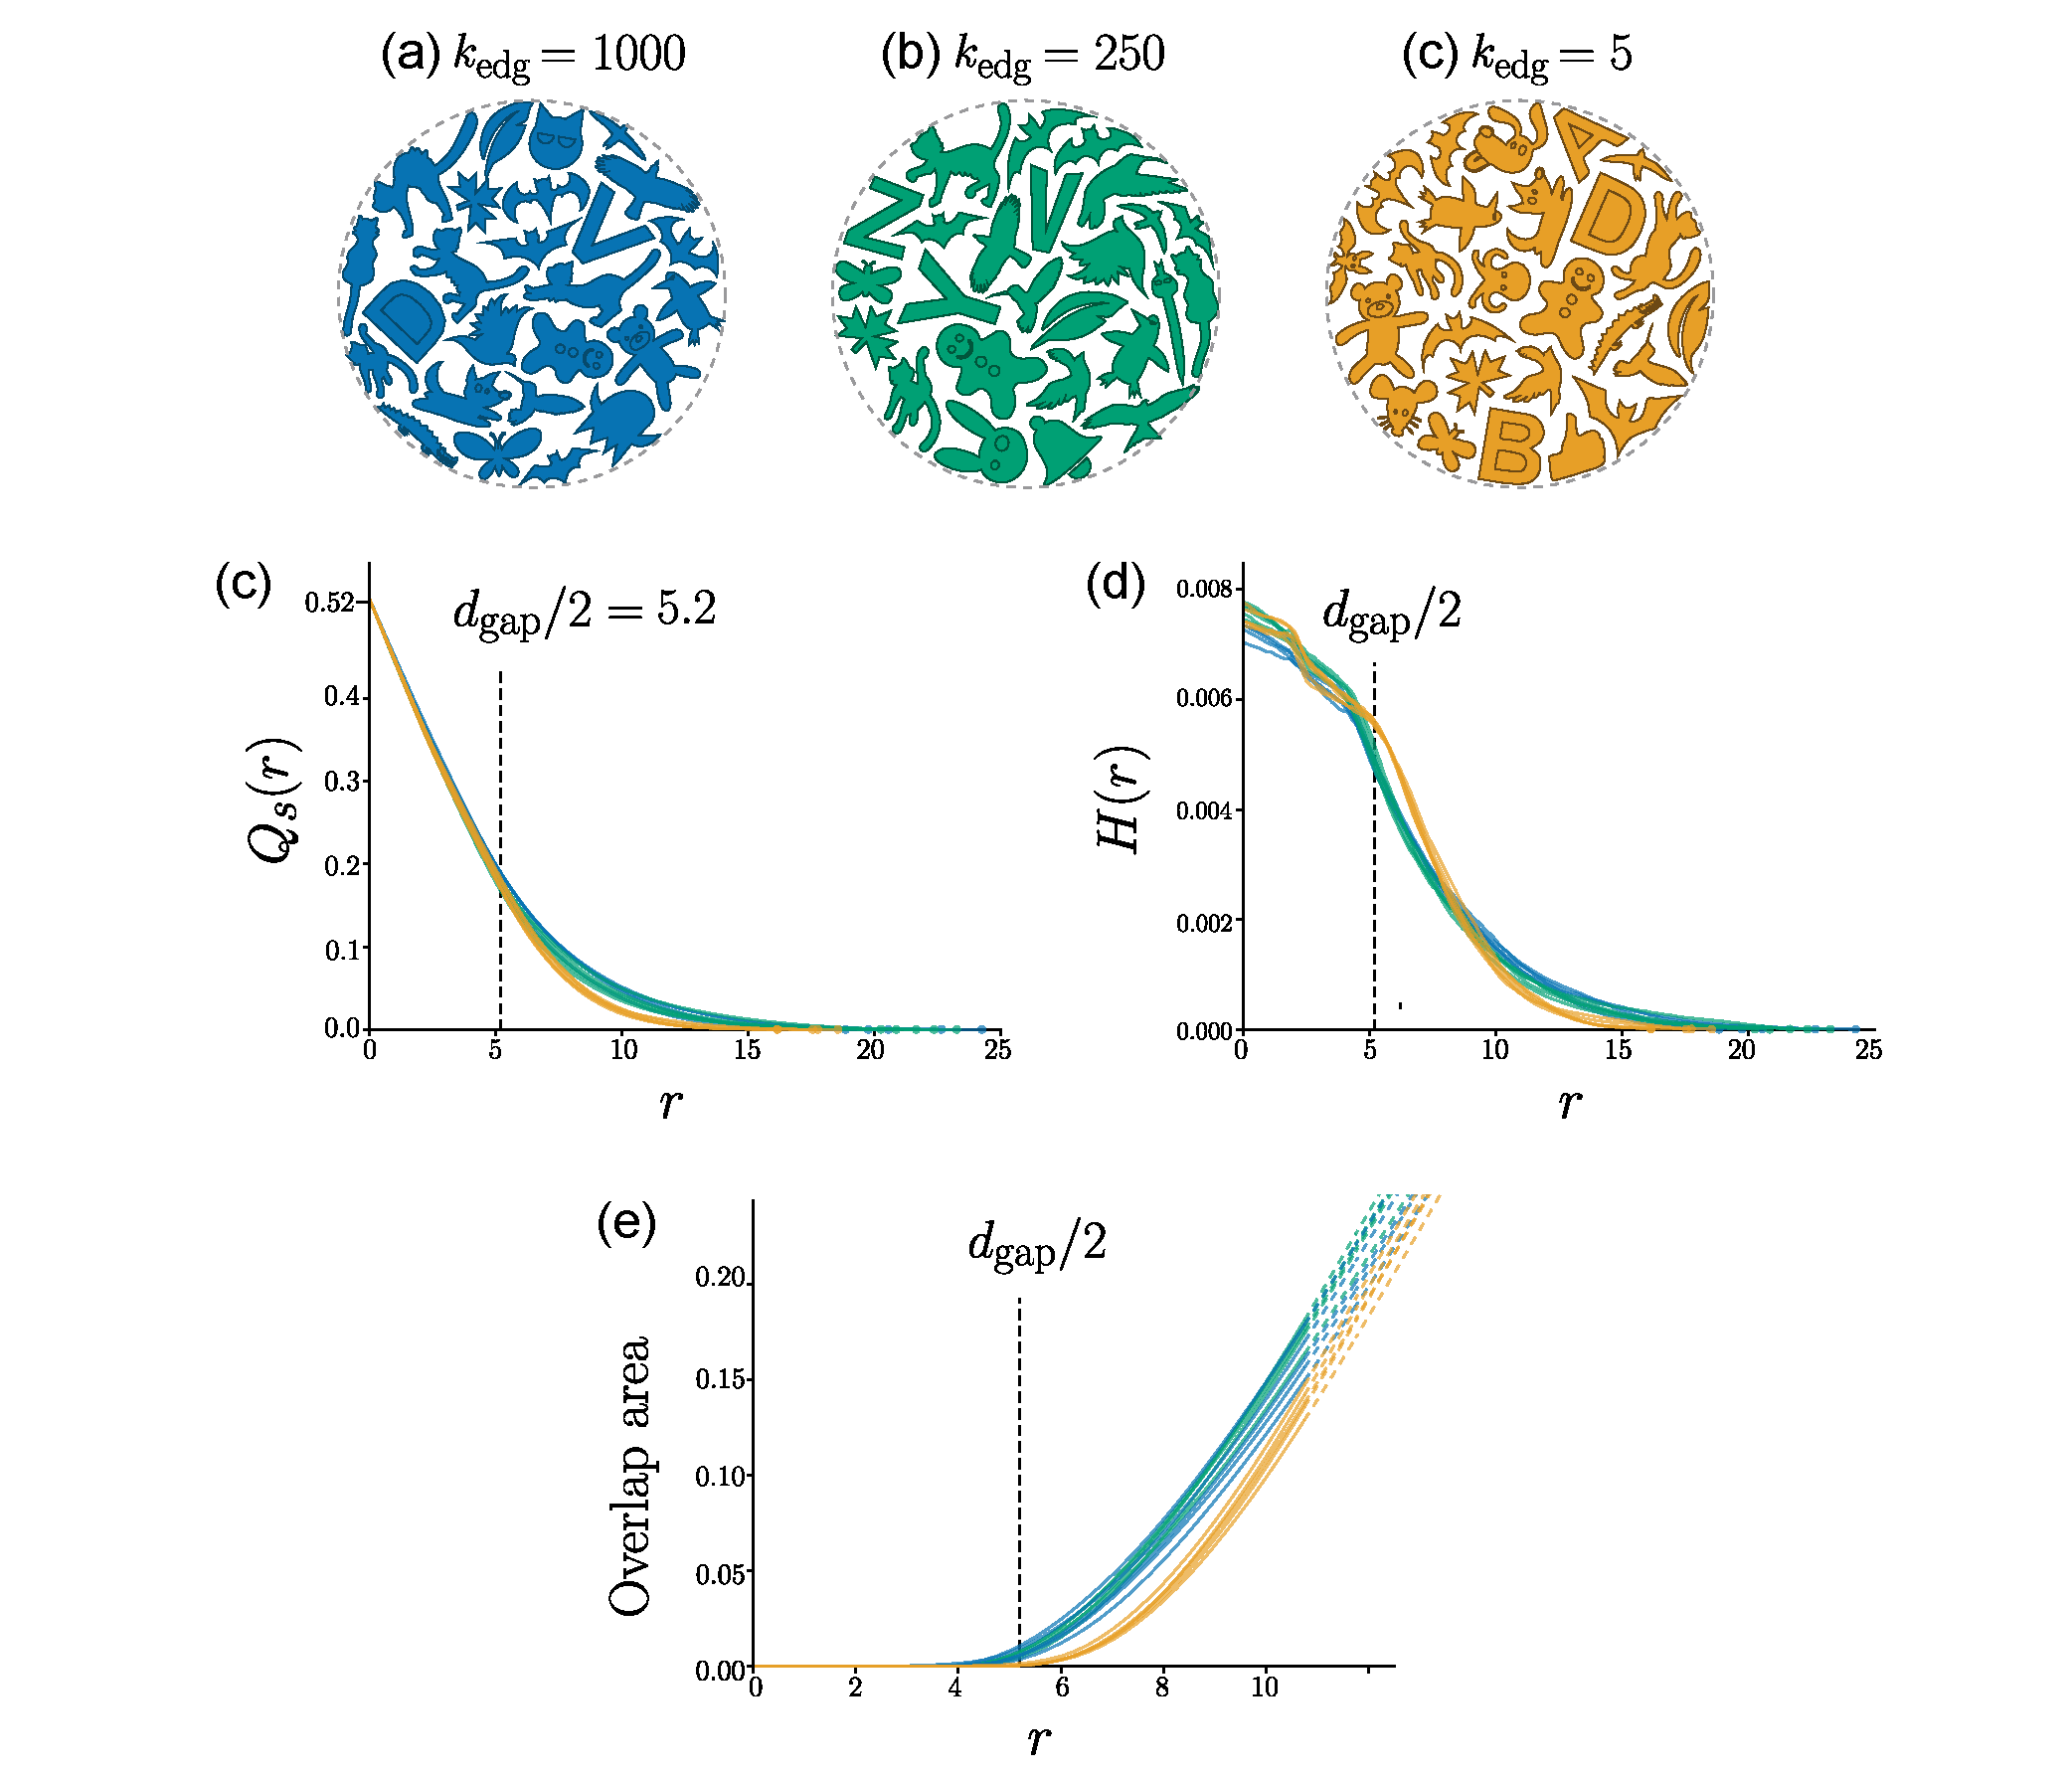
\includegraphics[width=1.0\textwidth]{figures/metrics/evaluation_big.pdf}
\caption[A demonstration of the effect of deformation \newline on the evenness of negative space]
{\label{fifteen_packings}
A demonstration of the effect of deformation on the evenness of negative space.  
The packings in (a), (b) and (c) are representative results using three values of the edge force strength $k_\mathrm{edg}$,
from rigid ($k_\mathrm{edg}=1000$) to moderate ($k_\mathrm{edg}=250$) to deformable ($k_\mathrm{edg}=5$).
We construct five random packings for each value of $k_\mathrm{edg}$, and plot their SCPs~(d), histograms~(e), and overlap functions~(f).
Packings with the most deformation have steeper and shorter SCPs, 
more histogram concentrations around $d_\mathrm{gap} / 2$, and lower overlap functions.
}
\end{figure}


 \newpage
%%%%%%%%%%%%%%%%%%%%%%%%%%%%%%%%%%%%%%%%%%%%%%%%%%%%%%%%%%
\section{Conclusions}
%%%%%%%%%%%%%%%%%%%%%%%%%%%%%%%%%%%%%%%%%%%%%%%%%%%%%%%%%%

\newtext{
The evenness of negative space is an indicator
of the quality of a packing. 
The more the elements interlock, the more even the negative space.
we validated our deformation-driven approach using overlap functions,
spherical contact probabilities, and histograms of distance transform.
A packing with a more even negative space has a steeper and shorter SCP, 
more histogram concentrations around $d_\mathrm{gap} / 2$, and a lower overlap function.}








